%------------------------------------------
% Szakdolgozat
% 
% 
% Varga Roland
%
% Konzulens: Magyar László
%------------------------------------------

\documentclass[12pt,a4paper,twoside]{article}
\usepackage{dissert}
% \renewcommand{\familydefault}{ptm}

\begin{document}
\pagenumbering{roman}
\author{Varga Roland}
\title{Ember és robot interakciójának demonstrációja\\
		Sakkozó iiwa robotkar}
%--Szennycímoldal-----------------------------------------
\newpage\thispagestyle{empty}
\begin{center}
     VARGA ROLAND\\
     SZAKDOLGOZAT
\end{center}
%--Sorozatcímoldal----------------------------------------
%\newpage\null\thispagestyle{empty}
\newpage\thispagestyle{empty}
\begin{center}
     BUDAPESTI MŰSZAKI ÉS GAZDASÁGTUDOMÁNYI EGYETEM\\
     GÉPÉSZMÉRNÖKI KAR\\
     MECHATRONIKA, OPTIKA ÉS GÉPÉSZETI INFORMATIKA TANSZÉK\\[1ex]
     \resizebox{2.5cm}{!}{
          
\includegraphics{figures/mogi.png}
     }\\[1ex]
     SZAKDOLGOZATOK
\end{center}
%--Címoldal-----------------------------------------------
%\newpage\null\thispagestyle{empty}
\newpage\thispagestyle{empty}
\begin{titlepage} %environment for unique titlepage design
\centering
\resizebox{4.5cm}{!}{
  
\includegraphics{bme}
}\\[1ex]
{\bf BUDAPESTI MŰSZAKI ÉS GAZDASÁGTUDOMÁNYI EGYETEM}\\
{\bf GÉPÉSZMÉRNÖKI KAR}\\
{\bf MECHATRONIKA, OPTIKA ÉS GÉPÉSZETI INFORMATIKA TANSZÉK}\\[3cm]

{\LARGE \scshape Varga Roland}\\[2ex]
{\Large SZAKDOLGOZAT}\\[2ex]
{\Large \bf Ember és robot kooperációjának demonstrálása\\
		Sakkozó iiwa robotkar segítségével}\\[2ex]
{\itshape Demonstrating human-robot collaboration\\
				With chess-playing iiwa robotic arm}\\[5cm]

\begin{tabularx}{\textwidth}{XXXX}
Konzulens: & Témavezető: \\
\hspace{0.75cm} \itshape Magyar László & \hspace{0.75cm} \itshape Dr. Czmerk András \\
\hspace{0.75cm} tesztmérnök & \hspace{0.75cm} egyetemi adjunktus \\
\end{tabularx}\\[4cm]

{\Large Budapest, 2018}
\end{titlepage}

%--Záradék és nyilatkozatok-------------------------------
%--Copyright oldal----------------------------------------
\newpage\null\thispagestyle{empty}
\newpage\thispagestyle{empty}
Szerzői jog \textcopyright ~Knyihár Gábor, 2018.\\[2cm]

\begin{center}
    \bf ZÁRADÉK
\end{center}


{\bf Ez a szakdolgozat elzártan kezelendő és őrzendő, a hozzáférése a vonatkozó szabályok szerint korlátozott, a dolgozat tartalmát csak az arra feljogosí-tott személyek ismerhetik.}

{\bf A korlátozott hozzáférés időtartamának lejártáig az arra feljogosítottakon kívül csak a korlátozást kérelmező személy vagy gazdálkodó szervezet írásos engedélyéjével rendelkező személy nyerhet betekintést a dolgozat tartalmába.}\\[0.5cm]

{\bf A hozzáférés korlátozása és a zárt kezelés 2023. év december hónap 
31. napján ér véget.}

%--Feladatkiírás lapja------------------------------------
\newpage\null\thispagestyle{empty}
\newpage\thispagestyle{empty}

%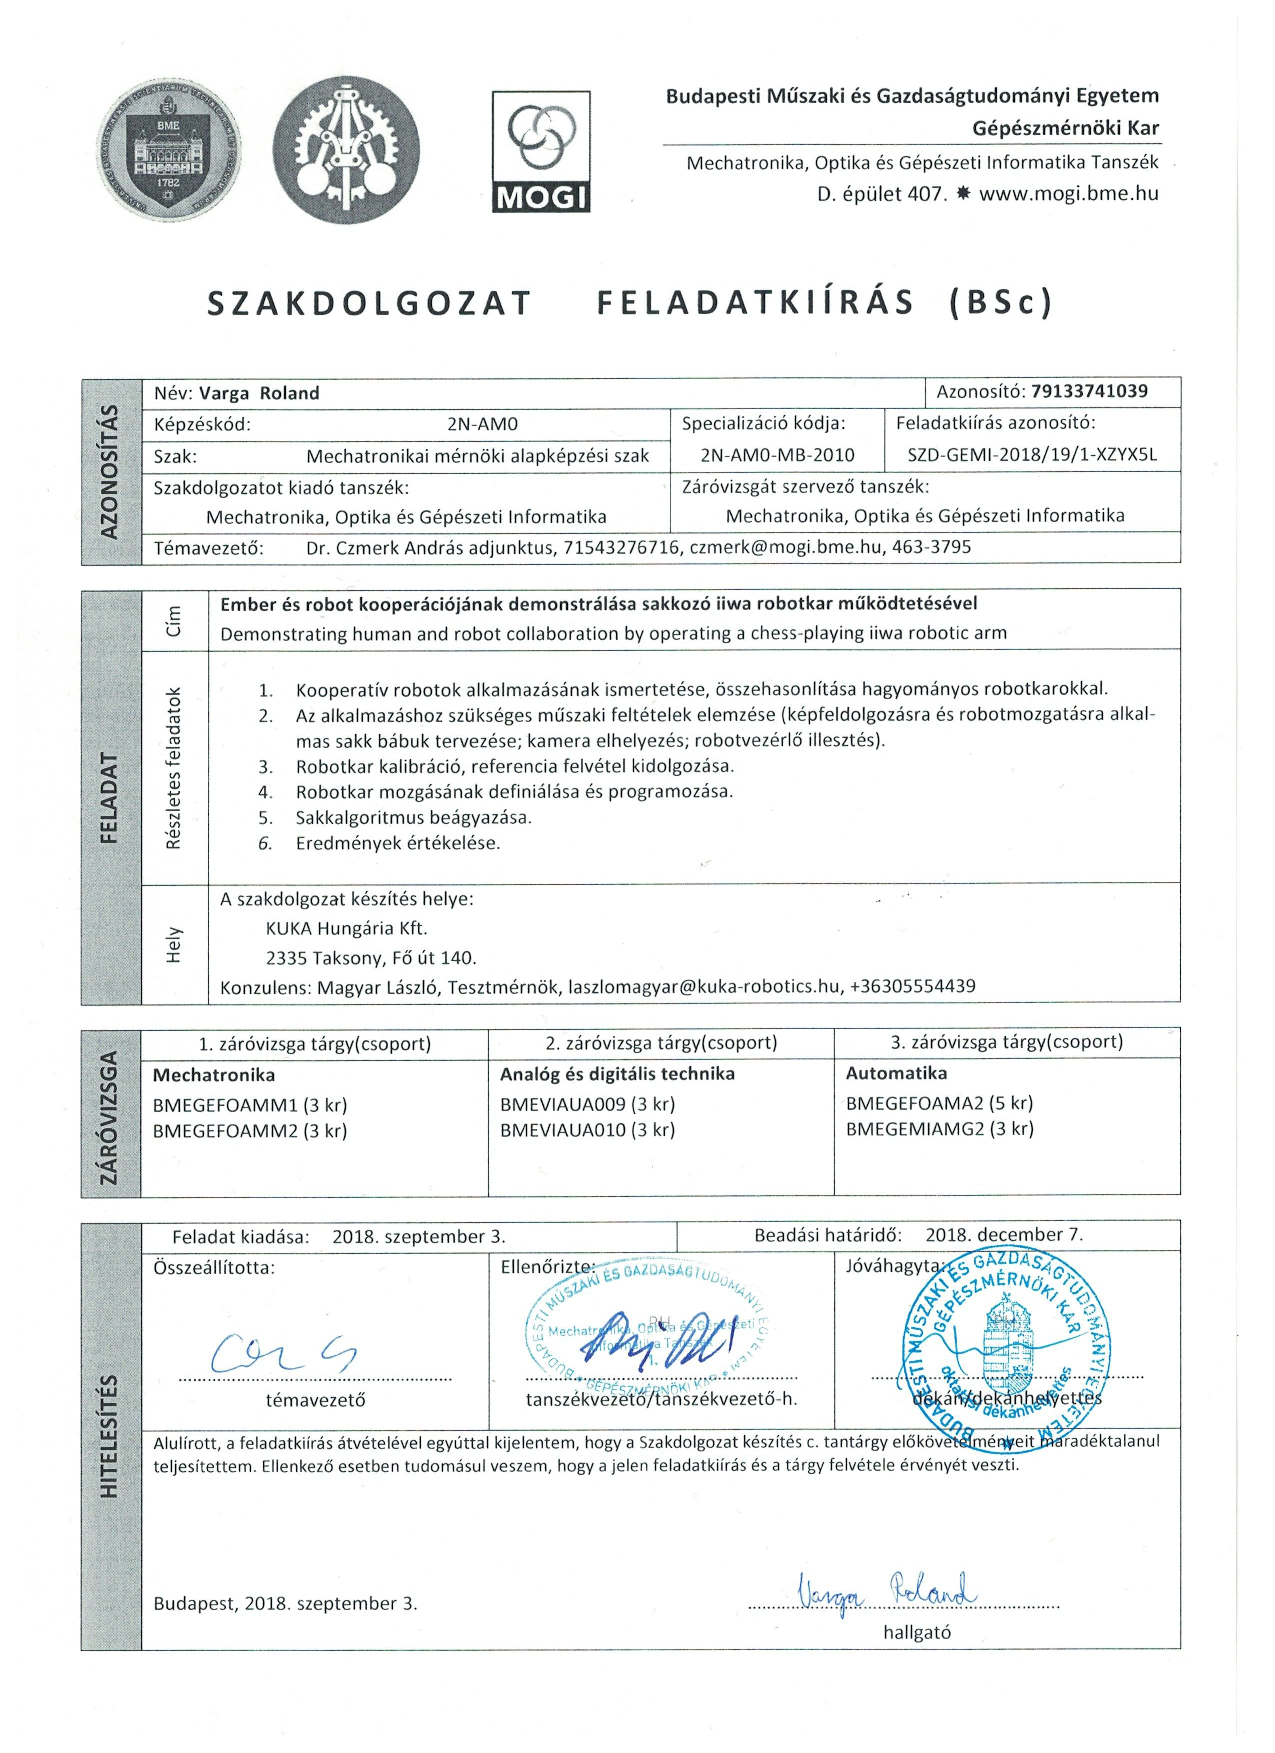
\includepdf[pages=-, offset=75 -75]{Figures/feladatkiiras.pdf}

%--Nyilatkozatok------------------------------------------
\newpage\null\thispagestyle{empty}
\newpage\thispagestyle{plain}
\begin{center}
    \Large \MakeUppercase{Nyilatkozatok}
\end{center}

{\centering \itshape Beadhatósági nyilatkozat \par}
A jelen szakdolgozat az üzem által elvárt szakmai színvonalnak mind tartalmilag, mind formailag megfelel, beadható.

Kelt, 

{\hspace{0.4\textwidth} Az üzem részéről:}\\[1cm]

{\hspace{0.6\textwidth} \itshape üzemi konzulens}\\[0.1cm]

{\centering \itshape Elfogadási nyilatkozat \par}
Ezen szakdolgozat a Budapesti Műszaki és Gazdaságtudományi Egyetem Gépészmérnöki Kara által a Diplomatervezési és Szakdolgozat feladatokra előírt valamennyi tartalmi és formai követelménynek, továbbá a feladatkiírásban előírtaknak maradéktalanul eleget tesz. E szakdolgozatot a nyilvános bírálatra és nyilvános előadásra alkalmasnak tartom. 

A beadás időpontja: \\[1cm]

{\hspace{0.62\textwidth} \itshape témavezető}\\[0.1cm]

{\centering \itshape Nyilatkozat önálló munkáról \par}
Alulírott, Varga Roland (XZYX5L), a Budapesti Műszaki és Gazdaságtudományi Egyetem hallgatója, büntetőjogi és fegyelmi felelősségem tudatában kijelentem és sajátkezű aláírásommal igazolom, hogy ezt a szakdolgozatot meg nem engedett segítség nélkül, saját magam készítettem, és dolgozatomban csak a megadott forrásokat használtam fel. Minden olyan részt, melyet szó szerint vagy azonos értelemben, de átfogalmazva más forrásból átvettem, egyértelműen, a hatályos előírásoknak megfelelően, a forrás megadásával megjelöltem.

{Budapest, 2018 ......................}\\[1cm]

{\hspace{0.6\textwidth} \itshape szigorló hallgató}

%--Tartalomjegyzék----------------------------------------
\newpage\null\thispagestyle{empty}
\newpage\pagestyle{empty}
\addtocontents{toc}{\protect\thispagestyle{empty}}
\tableofcontents

\pagenumbering{arabic}

%--Előszó-------------------------------------------------
\newpage
\thispagestyle{plain}
\setcounter{page}{1}
\subfile{sections/prolog}
%--Jelölések jegyzéke-------------------------------------
%\newpage\null\thispagestyle{empty}
%\newpage\thispagestyle{plain}
%\section*{Jelölések jegyzéke}

%A táblázatban a többször előforduló jelölések magyar és angol nyelvű elnevezése, valamint a fizikai mennyiségek esetén annak mértékegysége található. Az egyes mennyiségek jelölése – ahol lehetséges – %megegyezik hazai és a nemzetközi szak-irodalomban elfogadott jelölésekkel. A ritkán alkalmazott jelölések magyarázata első előfordulási helyüknél található.
%--Footer-------------------------------------------------
%\newpage\null\thispagestyle{empty}

%\include{boschfoot}

%--Köszönetnyílvánítás----------------------------------------------
\cleardoublepage
\thispagestyle{plain}
\subfile{sections/acknowledgement}

%--Bevezetés----------------------------------------------
\newpage
\pagestyle{fancy}
\subfile{sections/preamble}

%--Irodalomkutatás----------------------------------------
\clearpage
\subfile{sections/literature}
%---------------------------------------------------------

%--Tartalmi rész------------------------------------------
%--Robotkar mozgásának definiálása és programozása
	\clearpage
	\subfile{sections/projectdescription}
	%--A kamera kezelésével kapcsolatos csomag leírása
	\clearpage
	\subfile{sections/camerahandling}
	%--A bábuk kialakítása és a képfeldolgozási rész
	\clearpage
	\subfile{sections/imageprocessing}
	%--Sakkalgoritmus beágyazása
	\clearpage
	\subfile{sections/chess-algorithm}
	%--Robotkar kalibráció, referenciafelvétel kidolgozása
	\clearpage
	\subfile{sections/calibration}
	%--Robotkar mozgásának definiálása és programozása
	\clearpage
	\subfile{sections/motions}
	%--A megfogó vezérlése
	\clearpage
	\subfile{sections/grippercontrol}
	%--Eredmények értékelése
%	\clearpage
	\subfile{sections/results}
%---------------------------------------------------------

%--Összefoglalás------------------------------------------
\clearpage
\subfile{sections/summary-hu}
%---------------------------------------------------------

%--Angol összefoglalás------------------------------------
\clearpage \thispagestyle{empty}
\addcontentsline{toc}{section}{Abstract}
\subfile{sections/summary-en}
%---------------------------------------------------------

%--Források-----------------------------------------------
\newpage
\addcontentsline{toc}{section}{Hivatkozások}
\bibliographystyle{unsrt}
%\bibliographystyle{acm}
\bibliography{references}
%---------------------------------------------------------

%--Rövidítések jegyzéke----------------------------
%\newpage
%\addcontentsline{toc}{section}{Rövidítések jegyzéke}
%\begin{abbreviations}
%	\item[HRC]	\angol{Human Robot Collaboration}
%	\item[IoT]	\angol{Internet of Things}
%	\item[IoE]	\angol{Internet of Everything}
%	\item[TCP]	\angol{Tool Center Point}
%	\item[HRI]	\angol{Human-Robot Interaction}
%\end{abbreviations}
%-------------------------------------------------------

%--Függelékek--------------------------------------
\clearpage
%\appendix
\subfile{sections/appendix}

\end{document}